\chapter{Implementation} \label{chap: kalman implem}
The Kalman Filters were initially written in MatLab. However the static Kalman Filter was the only Kalman Filter that was tested on the quad-rotor. It was the only one that could be implemented due to the limited computational speed available on the micro-controller.

\section{Testing the Kalman Filter in MatLab} \label{sec: kalman filter responces}

The Kalman Filter was tested in simulation to observe its performance under high and low acceleration by means of comparison of attitude measured by the accelerometer and attitude measured by a potentiometer \footnote{In this case the potentiometer was taken to be the correct attitude as it was aligned along the axis of rotation of the quad-rotor. The potentiometer was a laboratory standard measurement device which produce an analog measurement with low noise, meaning all of the filters produced in the report could be tuned by means of this potentiometer reading.}. The Static and Kinematic Kalman Filters were designed and tested using m-files in MatLab, which can be seen in Appendix \ref{sec: static Kalman Filter} and \ref{sec: Kinematic Kalman Filter} respectively. The models used to estimate the orientation using the Static Kalman Filter are the same models used for the control of the quad-rotor and are presented in \eqref{eq: pitch model}, \eqref{eq: roll model}, \eqref{d2ydt2} and the model used for the Kinematic Kalman Filter was presented in \eqref{eq: rotation matrix related using the gyro readings}. In order for the filters to be tuned the noise of the accelerometer, gyroscope and magnetometer were modeled and after which a Kalman Filter was produced so an accurate estimate of the attitude could be acquired. Figure \ref{fig kalman filter comparison} clearly shows that the Kalman Filter gives a good estimate of the orientation and smoothing of the accelerometer data does indeed take place.


\begin{figure}[h]
	\centering
	\begin{subfigure}{0.32\textwidth}
		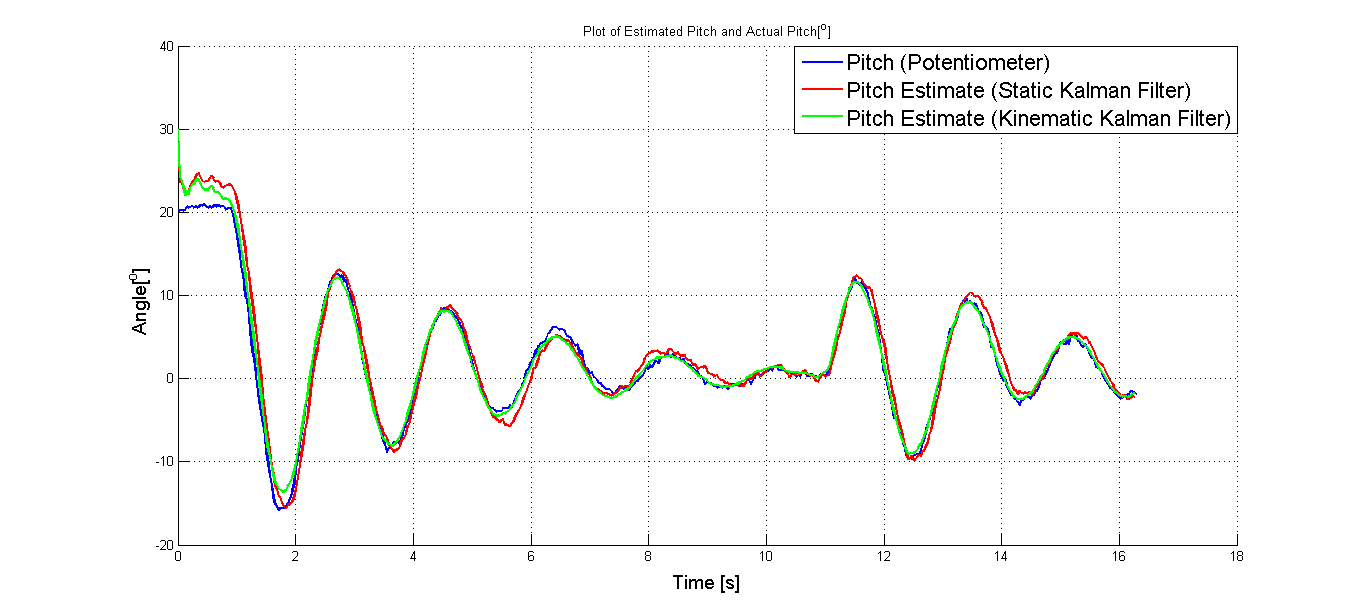
\includegraphics[width =0.36\paperwidth]{\DocRoot/images/Kalman_fitler_compare}
		\caption{Time domain comparison of Static and Kinematic Kalman Filter}
		\label{fg: Time domain comparison of Static and Kinematic Kalman Filter}
	\end{subfigure}%
	\hspace{3cm}
	\begin{subfigure}{0.32\textwidth}
		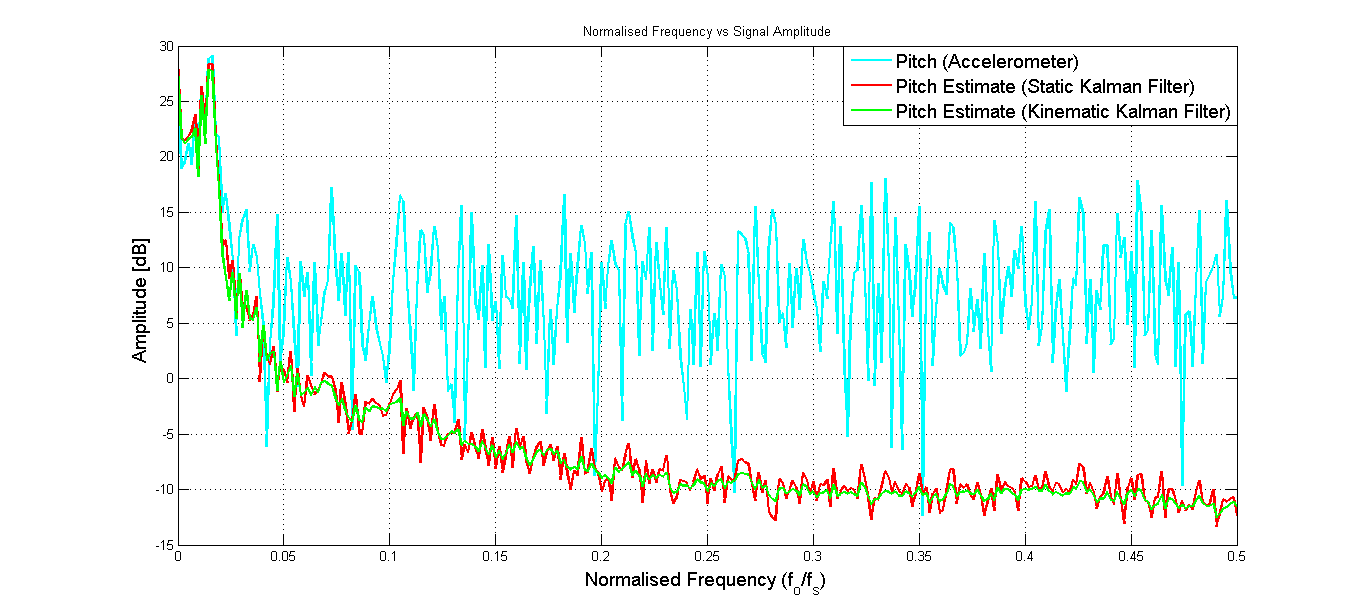
\includegraphics[width =0.36\paperwidth]{\DocRoot/images/fft_kalam_compare}
		\caption{Frequency domain comparison of Static and Kinematic Kalman Filter}
		\label{fg: Frequency domain comparison of Static and Kinematic Kalman Filter}
	\end{subfigure}

\caption{Comparison of Kalman Filters used during the Project}
\label{fig kalman filter comparison}	
\end{figure}

\section{Testing the Kalman Filter in Simulation}
To convert the Matrix Exponentiation function used in MatLab, approximations have to be made as the processing power required to calculate the Matrix Exponentiation in full is too great.

\subsection{Approximations Used}
So as to implement the Kinematic Kalman Filter on the micro-controller an approximation to the Matrix Exponential was made. The Matrix Exponential can be defined as follows:- 

\begin{equation}
e^{\underline{\bf X}} = \sum_{k=0}^{\infty}\frac{1}{k!}{\underline{\bf X}}^k
\label{eq: matrix exponential}
\end{equation}

Equation \ref{eq: matrix exponential} is an infinite series, thus, an approximation is required to implement the filter on the micro-controller.

\begin{equation}
e^{\gls{skewmatrix}\gls{ts}} = I + \gls{skewmatrix}\gls{ts} + \frac{(\gls{skewmatrix}\gls{ts})^2}{2!} + \dddot{}   +\frac{(\gls{skewmatrix}\gls{ts})^5}{5!}  
\end{equation}

It was not required to go beyond the $3^{th}$ term in the approximation of the matrix exponential since terms larger than the $3^{th}$ were of too small a magnitude to affect the result.



\section{Testing the Estimator with the Sensors}
Section \ref{sec: kalman filter responces} shows the Kalman Filters response in simulation. However, when estimating the orientation of the quad-rotor, the actual orientation was required to ensure the estimate produced by the filter was correct. This was achieved by placing the sensors on the quad-rotor, which in turn was mounted on a rig, which had potentiometers to measure the actual orientation. The rig was arranged so that the pitch and roll could not vary more than $\pm 30^o$. A picture of this arrangement can be seen in Figure \ref{Fig: test rig}. The \gls{noisecomatrix} was chosen by gathering data while the sensor was level and at rest. This data was called into MatLab where the \textit{cov} command was used to find the covariance of the accelerometer, gyroscope and magnetometer respectively. The \gls{noisecoplantmatrix} value for the Static Kalman Filter was difficult to acquire without flight data so it had to be approximated. As for the Kinematic Kalman Filter, the \gls{noisecoplantmatrix} was set to the covariance value of the gyroscope as the \gls{Transitionmatrix} of this filter is made from the gyroscope outputs. 


The code used to communicate with the \gls{9dof} was modified so that the potentiometer values could be read by means of an {ADC} on the micro-controller board. After the Micro-controller read the associated values (both \gls{9dof} values and potentiometer values) they were then recorded on a SD card so the data could be called into MatLab. This allowed post processing to be applied to the \gls{9dof} data. The \gls{noisecoplantmatrix} was adjusted until the potentiometer data matched the estimate produced by the Kalman Filter at both high and low accelerations.



\begin{figure}[h]
	\centering
	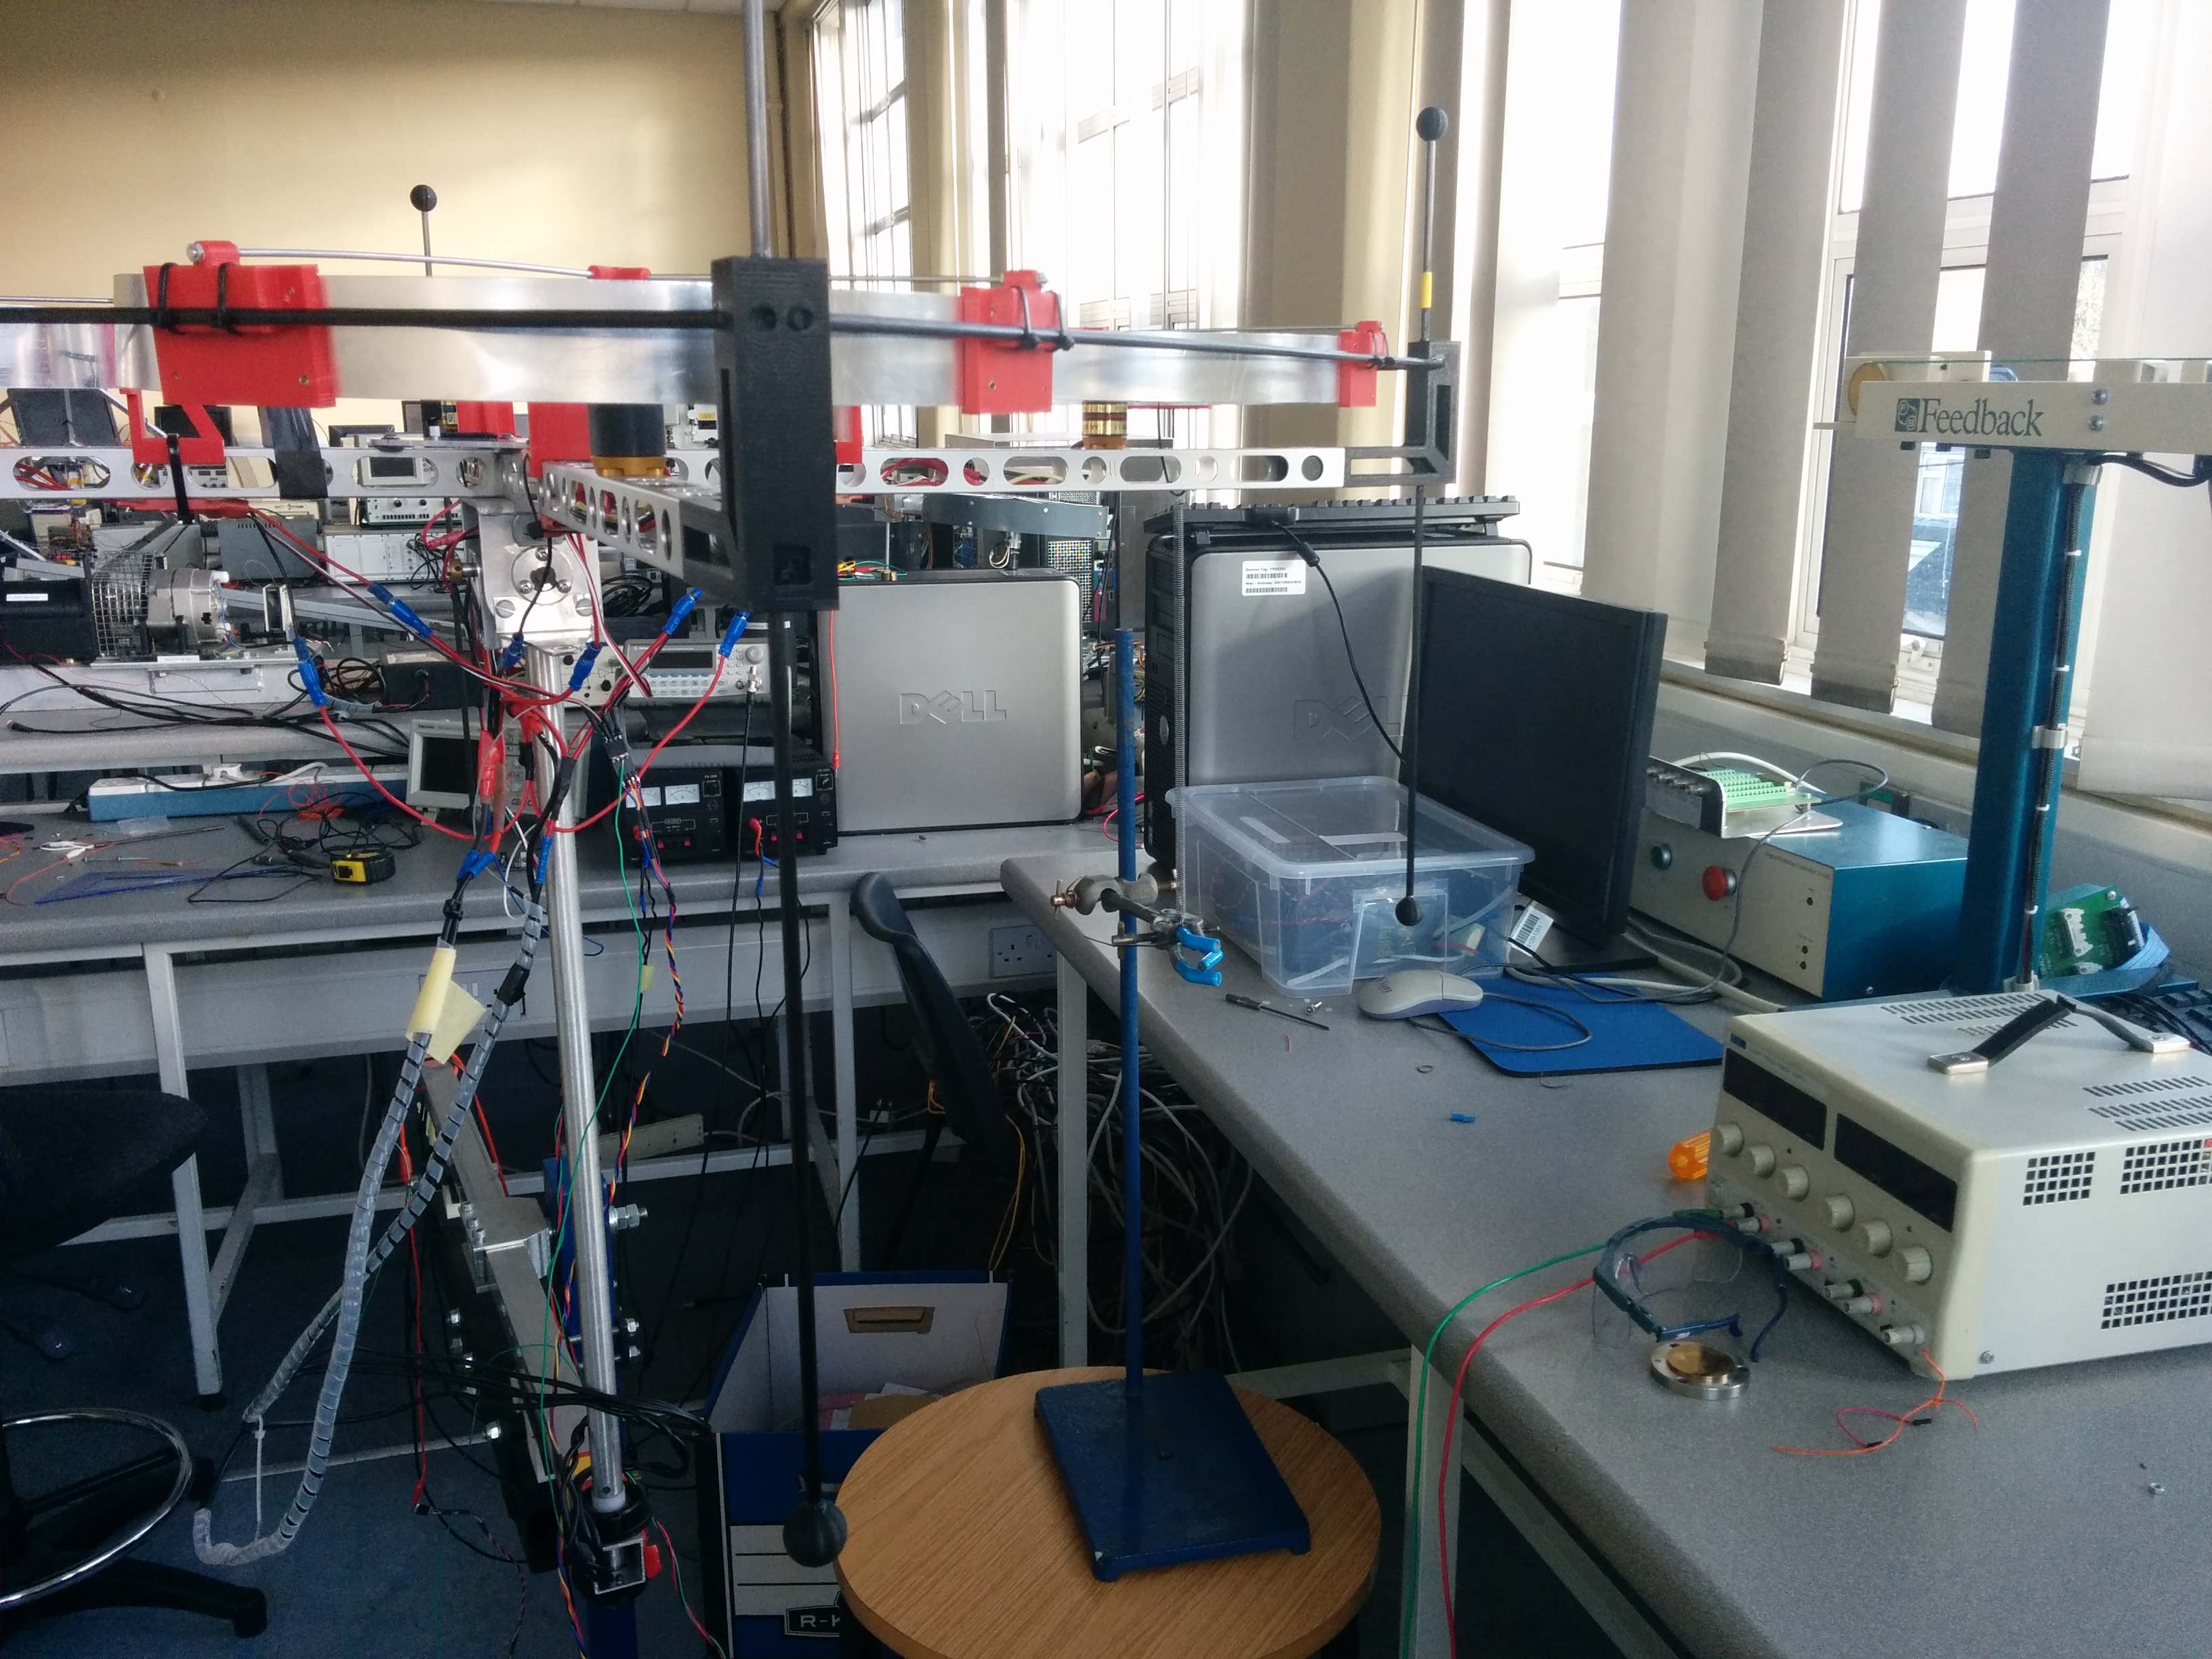
\includegraphics[width =0.7\paperwidth]{\DocRoot/images/quad_photo}
	\caption{Rig used to test the Kalman Filter}
	\label{Fig: test rig}
\end{figure}


\section{Tuning the Kalman Filter}
The Kalman Filter is often used as an estimator, but is widely known to be difficult to tune. Tuning the filter implies determining the \gls{noisecomatrix} and \gls{noisecoplantmatrix} matrices which control how the filter combines the model and the measurement to acquire an accurate estimate of the state vector. The accuracy of the filter's estimate depends on the \gls{noisecomatrix} and \gls{noisecoplantmatrix} matrices. Throughout the project many tuning methods were investigated, but the tuning method presented in \cite{gordon_paper} gave the best/desired results. The \gls{noisecomatrix} matrix can be estimated with ease, as the covariance of the data produced by the sensor while at rest can easily be found.

\subsubsection{Estimating the \gls{noisecomatrix} matrix}
As the accelerometer was thought to have a greater covariance at high accelerations (as the accelerometer also measures linear and angler acceleration) it was decided to test the device under high acceleration. In order to see if high acceleration components increased the covariance of the accelerometer data it was decided to gather data on the quad-rotor under high acceleration with motors on. It was found that the high acceleration components where lower than the noise floor produced by the vibrations due to the motors attached to the quad-rotor. The omission of the "high" high acceleration was possible as the magnitude of the angular acceleration of the quad-rotor is quite low. The covariance was found by means of the $cov()$ function in MatLab. Hence, the \gls{noisecomatrix} was calculated as follows:-

					\begin{equation}
					\gls{noisecomatrix}_a  = 		
					\left[\begin{array}{ccc}
					\mathrm{cov(\gls{roll})}       &                 0                          & 0\\ 
					0       & \mathrm{cov(\gls{pitch})}           & 0\\
					0         &                0                          &\mathrm{cov(\gls{yaw})}
					\end{array} \right]
					\end{equation}


\subsubsection{Estimating the \gls{noisecoplantmatrix} matrix}

 Calculating the \gls{noisecoplantmatrix} matrix proved to be quite a difficult task. Very little actual information regrading the noise present in the states was known. However, since \gls{noisecoplantmatrix} was difficult to calculate without flight data it was decided to use a binary search using the ratio of \gls{noisecoplantmatrix}/\gls{noisecomatrix} as it was shown in \cite{gordon_paper} that this type of tuning could lead to an optimal response. In this tuning process the \gls{noisecomatrix} was set to the theoretical value and \gls{noisecoplantmatrix} was adjusted by means of a binary search, thus a filter signal similar to the potentiometer value was found. A similar approach was used to tune the Kinematic Kalman Filter, except some initial knowledge was known about the \gls{noisecoplantmatrix} as the transition matrix of this filter was made up solely of the gyroscope values. This allowed the \gls{noisecoplantmatrix} matrix for this filter to be set to the covariance values of the gyroscope. This approach produced almost identical results to the Static Kalman Filter with little tuning, but in order to improve the filtering of the Kinematic Kalman Filter a binary search was also used to improve the estimation of this filter and the results of both Kalman Filters can be seen in figure \ref{fig kalman filter comparison}.                                                                                                                                                                                                                                                                                                                                                                                                                                                                                                                                                                                                                                                                                                                                                                                                                                                                                                                                                                                                                                                                                                                                                                                                          
